\input ../SlidePreamble
\input ../preamble

\begin{document}

{\Huge

  \centerline{\bf TTIC 31230, Fundamentals of Deep Learning}
  \bigskip
  \centerline{David McAllester, Winter 2019}
  \vfill
  \centerline{Controlling Gradients}
  \vfill
  \vfill
  \centerline{Vanishing and Exploding Gradients}
  \vfill
  \centerline{Initialization}
  \vfill
  \centerline{Batch Normalization}
  \vfill
  \centerline{Residual Networks}
  \vfill
  \centerline{Gated RNNs}

\slide{The Expressive Power of DNNs}

Linear Threshold units generalize logical operations.

\vfill
Consider Boolean Values $P,Q$ --- numbers that are either close to 0 or close to 1.

\vfill
\begin{eqnarray*}
P \wedge Q & \approx & \sigma(100*P + 100* Q -150) \\
\\
P \vee Q & \approx & \sigma(100*P + 100* Q -50) \\
\\
\neg P & \approx & \sigma(100*(1-P) - 50)
\end{eqnarray*}

\vfill
DNNs generalize digital circuits.

\slide{DNNs are Expressive and Trainable}

{\color{red} Universality Assumption:} DNNs are universally expressive (can model any function) and trainable (the desired function can be found by SGD).

\vfill
The Universality assumption is clearly false but can still guide architecture design.

\vfill
But equally expressive architectures differ in trainability.  This lecture is on trainability.

\slide{Vanishing and Exploding Gradients}
~
\vfill
\centerline{Causes of Vanishing and Exploding Gradients:}
\vfill
\centerline{Activation function saturation}
\vfill
\centerline{Repeated multiplication by network weights}
\vfill

\slide{Activation Function Saturation}

Consider the sigmoid activation function $1/(1+ e^{-x})$.

\vfill
\centerline{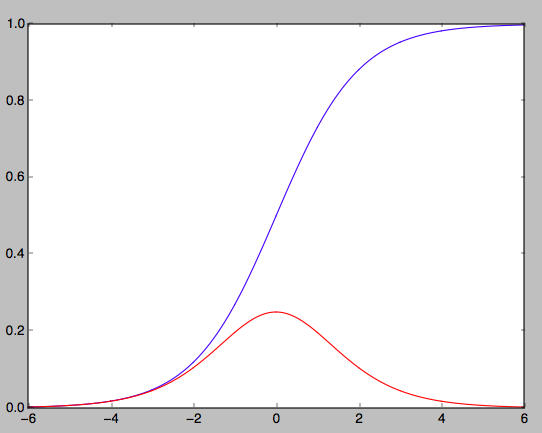
\includegraphics[width= 4.0in]{../images/sigmoid2}}


\vfill
The gradient of this function is quite small for $|x| > 4$.

\vfill
In deep networks backpropagation can go through many sigmoids and
the gradient can ``vanish''

\slide{Activation Function Saturation}

$\mathrm{Relu}(x) = \max(x,0)$

\vfill
\centerline{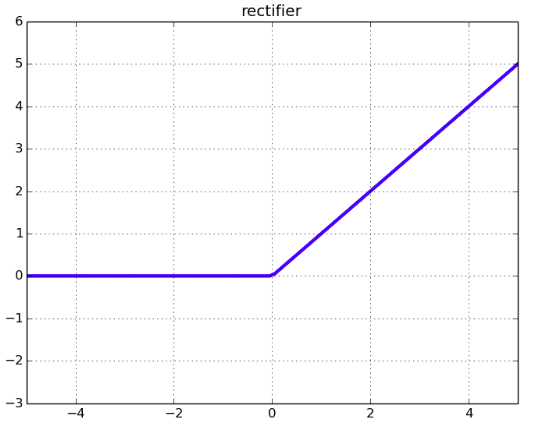
\includegraphics[width= 4.0in]{../images/relu}}

\vfill
The Relu does not saturate at positive inputs (good) but is completely saturated at negative inputs (bad).

\vfill
Alternate variations of Relu still have small gradients at negative inputs.

\slide{Repeated Multiplication by Network Weights}

Consider a deep CNN.

$$L_{i+1} = \mathrm{Relu}(\mathrm{Conv}(\Phi_i,L_i))$$

\vfill
For $i$ large, $L_i$ has been multiplied by many weights.

\vfill
If the weights are small then the neuron values, and hence the weight gradients, decrease exponentially with depth. {\bf Vanishing Gradients.}

\vfill
If the weights are large, and the activation functions do not saturate, then the neuron values, and hence the weight gradients,
increase exponentially with depth. {\bf Exploding Gradients.}

\slide{Methods for Maintaining Gradients}

\centerline{Initialization}

\vfill
\centerline{Batch Normalization}

\vfill
\centerline{Highway Architectures (Skip Connections)}

\slide{Methods for Maintaining Gradients}

\centerline{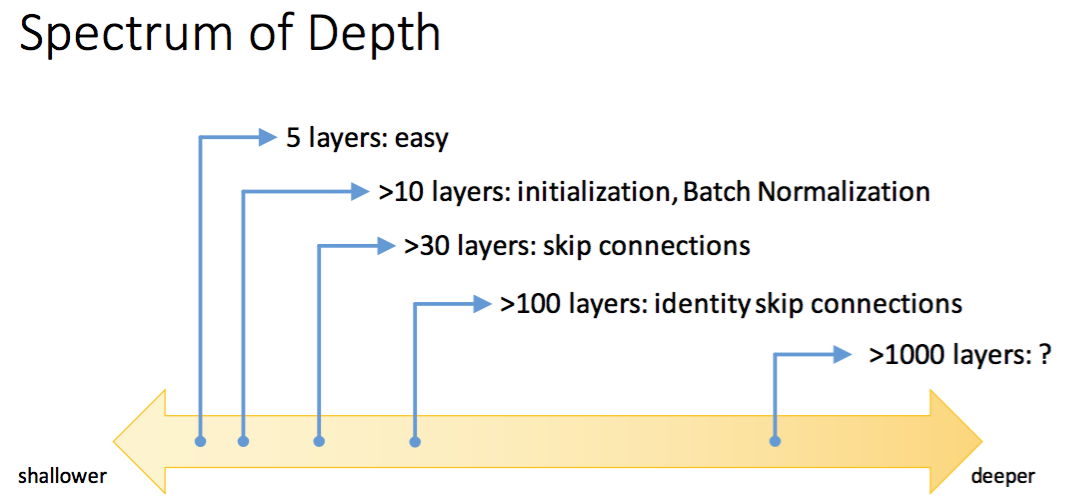
\includegraphics[width = 9in]{../images/DepthSpectrum}}

\centerline{\large Kaiming He}

\slide{}
\centerline{\bf Initialization}
\vfill

\slide{Xavier Initialization}

Initialize a weight matrix (or tensor) to preserve zero-mean unit variance distributions.

\vfill
If we assume $x_i$ has unit mean and zero variance then we want

\vfill
$$y_j = \sum_{j=0}^{N-1} x_i w_{i,j}$$

\vfill
to have zero mean and unit variance.

\vfill
Xavier initialization randomly sets $w_{i,j}$ to be uniform in the interval $\left(-\sqrt{\frac{3}{N}},\;\sqrt{\frac{3}{N}}\right)$.

\vfill
Assuming independence this gives zero mean and unit variance for $y_j$.

\slide{He Initialization}

A Relu nonlinearity reduces the variance.

\vfill
Before a Relu nonlinearity it seems better to use the larger interval $\left(-\sqrt{\frac{6}{N}},\;\sqrt{\frac{6}{N}}\right)$.

\slide{}
\centerline{\bf Batch Normalization}
\vfill

\slide{Normalization}
Given a tensor $x[b,j]$ we define $\tilde{x}[b,j]$ as follows.

\begin{eqnarray*}
  \hat{\mu}[j] & = & \frac{1}{B} \sum_b\;x[b,j] \\
  \\
  \\
  \hat{\sigma}[j] & = & \sqrt{\frac{1}{B-1} \sum_b (x[b,j]-\hat{\mu}[j])^2} \\
  \\
  \\
  \tilde{x}[b,j]& = & \frac{x[b,j] - \hat{\mu}[j]}{\hat{\sigma}[j]}
\end{eqnarray*}


\vfill
At test time a single fixed estimate of $\mu[j]$ and $\sigma[j]$ is used.

\slide{Spatial Batch Normalization}

For CNNs we convert a tensor $x[b,x,y,j]$ to $\tilde{x}[b,x,y,j]$ as follows.

\begin{eqnarray*}
  \hat{\mu}[j] & = & \frac{1}{BXY} \sum_{b,x,y}\;x[b,x,y,j] \\
  \\
  \\
  \hat{\sigma}[j] & = & \sqrt{\frac{1}{BXY-1} \sum_{b,x,y} (x[b,x,y,j]-\hat{\mu}[j])^2} \\
  \\
  \\
  \tilde{x}[b,x,y,j]& = & \frac{x[b,x,y,j] - \hat{\mu}[j]}{\hat{\sigma}[j]}
\end{eqnarray*}

\slide{Adding an Affine Transformation}

$$\breve{x}[b,x,y,j] = \gamma[j] \tilde{x}[b,x,y,j] + \beta[j]$$

\vfill
Here $\gamma[j]$ and $\beta[j]$ are parameters of the batch normalization.

\vfill
This allows the batch normlization to learn an arbitrary affine transformation (offset and scaling).

\vfill
It can even undo the normaliztion.

\slide{Batch Normalization}

Batch Normalization appears to be generally useful in CNNs but is not always used.

\vfill
Not so successful in RNNs.

\vfill
It is typically used just prior to a nonlinear activation function.

\vfill
It is intuitively justified in terms of ``internal covariate shift'':
as the inputs to a layer change the zero mean unit variance property underlying Xavier initialization are maintained.

\ignore{
\slide{Normalization Interacts with SGD}

Consider backpropagation through a weight layer.

\begin{eqnarray*}
  y.\mathrm{value}[\cdots] & \pluseq & w.\mathrm{value}[\cdots]\;x.\mathrm{value}[\dots] \\
  \\
  \\
  w.\mathrm{grad}[\cdots] & \pluseq & y.\mathrm{grad}[\cdots]\;x.\mathrm{value}[\cdots]
\end{eqnarray*}

\vfill
Replacing $x$ by $x/\hat{\sigma}$ seems related to RMSProp for the update of $w$.

\slide{The Simple Normalization Conjecture}

A simple normalization layer $y = \alpha (x + \beta)$ can be used in place of batch normalization as long $\beta$ is initialized to $-\hat{\mu}$
and $\alpha$ is initialized to $1/\hat{\sigma}$.

\vfill
Here $\hat{\mu}$ and $\hat{\sigma}$ should be computed only after earlier normalizations have been properly initialized.
}

\vfill
\eject
~ \vfill
\centerline{\bf Highway Architectures (Skip Connections)}
\vfill
\vfill

\slide{Deep Residual Networks (ResNets) by Kaiming He 2015}

\vfill
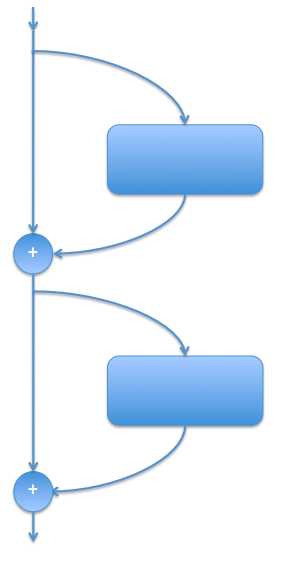
\includegraphics[width= 2.5in]{../images/resnet}
\hfill \begin{minipage}[b]{4in}
  A ``skip connection'' is adjusted by a ``residual correction''

  \bigskip
  The skip connections connects input to output directly and hence preserves gradients.

  \bigskip
  ResNets were introduced in late 2015 (Kaiming He et al.) and revolutionized computer vision.
\end{minipage}

\anaslideplain{Simple Residual Skip Connections in CNNs (stride 1)}

\medskip
\begin{eqnarray*}
R_{\color{red} \ell+1}[B,X,Y,J] & = & \mathrm{Conv}(W_{\color{red} \ell+1}[X,Y,J,J],B_{\color{red} \ell+1}[J],L_{\color{red} \ell}[B,X,Y,J]) \\
\\
\mathrm{for}\;b,x,y,j\;\;\;\;\;\;\;\\
L_{\color{red} \ell+1}[b,x,y,j] & = & L_{\color{red}\ell}[b,x,y,j] + R_{\color{red} \ell+1}[b,x,y,j]
\end{eqnarray*}

\vfill I will use capital letter indeces to denote entire tensors and lower case letters for particular indeces.

\anaslide{Simple Residual Skip Connections in CNNs (stride 1)}

\medskip
\begin{eqnarray*}
R_{\color{red} \ell+1}[B,X,Y,J] & = & \mathrm{Conv}(W_{\color{red} \ell+1}[X,Y,J,J],B_{\color{red} \ell+1}[J],L_{\color{red} \ell}[B,X,Y,J]) \\
\\
\mathrm{for}\;b,x,y,j\;\;\;\;\;\;\;\\
L_{\color{red} \ell+1}[b,x,y,j] & = & L_{\color{red}\ell}[b,x,y,j] + R_{\color{red} \ell+1}[b,x,y,j]
\end{eqnarray*}

\vfill Note that in the above equations $L_{\color{red} \ell}[B,X,Y,J]$ and $R_{\color{red} \ell+1}[B,X,Y,J]$ are the same shape.
\vfill
In the actual ResNet $R_{\color{red} \ell+1}$ is computed by two or three convolution layers.

\slideplain{Handling Spacial Reduction}

Consider $L_{\color{red} \ell}[B,X_{\color{red} \ell},Y_{\color{red} \ell},J_{\color{red} \ell}]$ and $R_{\color{red} \ell+1}[B,X_{\color{red} \ell+1},Y_{\color{red} \ell+1},J_{\color{red} \ell+1}]$
\begin{eqnarray*}
X_{\color{red} \ell+1} & = & X_{\color{red} \ell}/s \\
Y_{\color{red} \ell+1} & = & Y_{\color{red} \ell}/s \\
J_{\color{red} \ell+1} & \geq &  J_{\color{red} \ell}
\end{eqnarray*}


\vfill
In this case we construct $\tilde{L}_{\color{red} \ell +1 }[B,X_{\color{red} \ell +1},Y_{\color{red} \ell+1},J_{\color{red}\ell +1}]$

\begin{eqnarray*}
\mathrm{for}\;b,x,y,j\;\;\tilde{L}_{\color{red} \ell+1}[b,x,y,j] & = & \left\{\begin{array}{ll} L_{\color{red} \ell}[b,s*x,s*y,j] & \mbox{for $j < J_{\color{red} \ell}$} \\ 0 & \mbox{otherwise} \end{array}\right.\\
\\
L_{\color{red} \ell+1}[B,X_{\color{red} \ell +1},Y_{\color{red} \ell+1},J_{\color{red}\ell +1}] & = & \tilde{L}_{\color{red} \ell+1}[B,X_{\color{red} \ell +1},Y_{\color{red} \ell+1},J_{\color{red}\ell +1}] \\
& & + R_{\color{red} \ell+1}[B,X_{\color{red} \ell +1},Y_{\color{red} \ell+1},J_{\color{red}\ell +1}]
\end{eqnarray*}

\slide{Resnet32}

\centerline{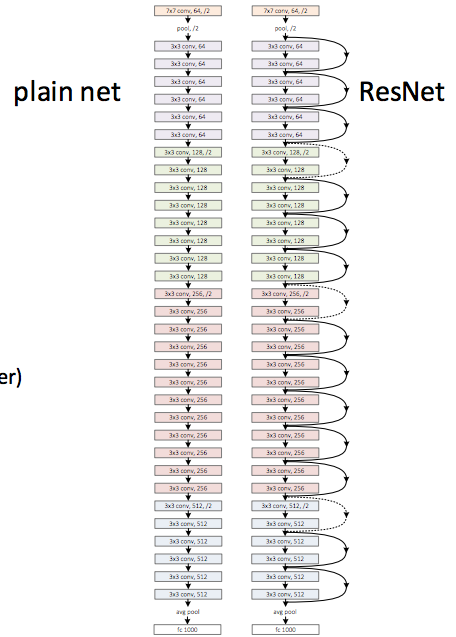
\includegraphics[height= 5.5in]{../images/ResnetStack} {\large [Kaiming He]}}


\slideplain{Deeper Versions use Bottleneck Residual Paths}
We reduce the number of channels to $K < J_{\color{red} \ell}$ before doing the convolution.

{\huge
\begin{eqnarray*}
A_{\color{red} \ell}[B,X_{\color{red} \ell},Y_{\color{red} \ell},K] & = & \mathrm{Conv}'(\Phi_{\color{red} \ell}^A{\color{red} [1,1,J_{\color{red} \ell},K]},L_{\color{red} \ell}[B,X_{\color{red} \ell},Y_{\color{red} \ell},J_{\color{red} \ell}]) \\
\\
B_{\color{red} \ell}[B,X_{\color{red} \ell+1},Y_{\color{red} \ell+1},K] & = & \mathrm{Conv}'(\Phi_{\color{red} \ell}^B{\color{red}[3,3,K,K]},A_{\color{red} \ell}[B,X_{\color{red} \ell},Y_{\color{red} \ell},K],\;\mathrm{stride}\;s) \\
\\
R_{\color{red} \ell+1}[B,X_{\color{red} \ell+1},Y_{\color{red} \ell+1},J_{\color{red} \ell+1}] & = & \mathrm{Conv}'(\Phi_{\color{red} \ell}^R{\color{red} [1,1,K,J_{\color{red} \ell+1}]},B_{\color{red} \ell}[B,X_{\color{red} \ell+1},Y_{\color{red} \ell+1},K]) \\
\\
L_{\color{red} \ell+1} & = & \tilde{L}_{\color{red} \ell+1} + R_{\color{red} \ell+1}
\end{eqnarray*}
}

\vfill
Here $\mathrm{CONV}'$ may include batch normalization and/or an activation function.

\slide{A General Resdual Connection}

$${\color{red} y = \tilde{x} + R(x)}$$

\vfill
Where $\tilde{x}$ is either $x$ or a version of $x$ adjusted to match the shape of $R(x)$.

\slide{DenseNet}

For {\color{red} $u[I]$} and {\color{red} $v[J]$} we let {\color{red} $(u;w)[I+J]$} denote vector concatenation.
\vfill
$$(u;v)[k] - \left\{\begin{array}{l} u[k]\;\mbox{for $k < J$} \\ v[k-I] \;\mbox{otherwise} \end{array}\right.$$

\vfill
$$\mbox{for}\;b,x,y\;\;L_{\color{red} \ell + 1}[b,x,y,J_{\color{red} \ell} + J_{\color{red} R}] = L_\ell[b,x,y,J_{\color{red} \ell}];R[b,x,y,J_{\color{red} R}]$$

\slide{Deep Residual Networks}

\vfill
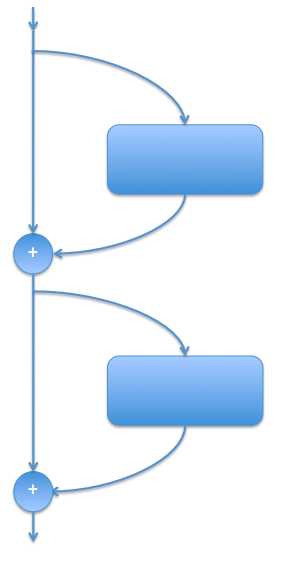
\includegraphics[width= 2.5in]{../images/resnet}
\hfill \begin{minipage}[b]{4in} As with most of deep learning, not much is known about what resnets are actually doing.
  
  \bigskip
  \bigskip
  For example, different residual paths might update disjoint channels making the networks shallower than they look.

  \bigskip
  \bigskip
  They are capable of representing very general circuit topologies.
\end{minipage}

\slideplain{}
\vfill
\centerline{Recurrent Neural Networks (RNNs)}
\vfill
\vfill

\slide{Vanilla RNNs}



\centerline{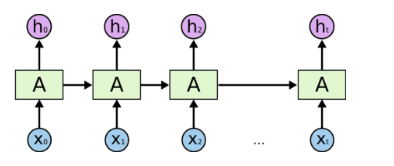
\includegraphics[width=3.5in]{../images/RNN}}
\centerline{{\large [Christopher Olah]}}

We use two input linear threshold units.

{\huge
$${\color{red} h_{t+1}[b,j]} = \sigma\left(\left(\sum_i\;W^{h,h}[i,j]{\color{red} h_t[b,i]}\right) + \left(\sum_k W^{x,h}[k,j]{\color{red} x_t[b,k]}\right) - B[j]\right)$$
}
\vfill
$$\mathrm{Parameter}\;{\color{red} \Phi = (W^{h,h}[J,J],\;W^{x,h}[K,J],\;B[J])}$$


\slide{Time as Depth}

\centerline{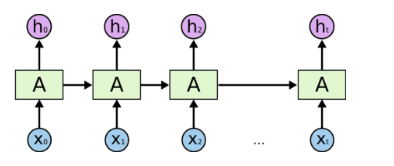
\includegraphics[width=3.5in]{../images/RNN}}
\centerline{{\large [Christopher Olah]}}

\vfill
We would like the RNN to {\color{red} remember and use} information from much earlier inputs.


\vfill
All the issues with depth now occur through time.

\vfill
However, for RNNs {\color{red} at each time step we use the same model parameters.}

\vfill
In CNNs {\color{red} at each layer uses its own model parameters.}

\slide{Exploding and Vanishing Gradients}

\vfill
If we avoid saturation of the activation functions then we get exponentially growing or shrinking eigenvectors of the weight matrix.

\vfill
Note that if the forward values are bounded by sigmoids or tanh then they cannot explode.

\vfill
However the gradients can still explode.

\slide{Exploding Gradients: Gradient Clipping}

\vfill
We can dampen the effect of exploding gradients by clipping them before applying SGD.

\vfill
$$W.\mathrm{grad} = \left\{\begin{array}{l} W.\mathrm{grad} \;\;\;\mbox{if $||W.\mathrm{grad}|| \leq n_{\mathrm{max}}$} \\
                                                      \\ \\
                                                      n_{\mathrm{max}} \; W.\mathrm{grad} / ||W.\mathrm{grad}|| \;\; \mbox{otherwise}
\end{array} \right.$$

\vfill
See {\tt torch.nn.utils.clip\_grad\_norm}

\slide{Skip Connections Through Time}

\centerline{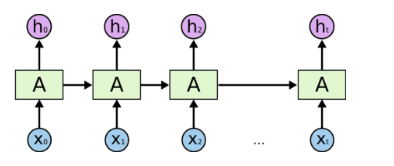
\includegraphics[width=3.5in]{../images/RNN}}
\centerline{{\large [Christopher Olah]}}

\vfill
We would like to add {\color{red} residual connections through time}.

\vfill
However, We have to handle the fact that the same model parameters are used at every time step.

\slide{Gated Skip Connections}


$$\begin{array}{lrcl}
\mbox{Residual Skip:} & L_{\ell+1} & = & {\color{red} \tilde{L}_\ell} + R_{\color{red} \Phi_{\ell+1}}({\color{red} L_\ell})
\end{array}$$
\vfill
Here ${\color{red} \Phi_{\ell+1}}$ controls data independent data flow.

\vfill
$$\begin{array}{lrcl}
\mbox{Gated Skip:} & h_{t+1} & = & G_t\odot {\color{red} h_t} + (1-G_t)\odot R_{\color{red} \Phi}(x_t,{\color{red} h_t}) \\
\end{array}$$

\vfill
\begin{eqnarray*}
(G\odot h)[b,j] & = & G[b,j] * h[b,j] \\
\\
(1-G_t)[b,j] & = & 1-G_t[b,j]
\end{eqnarray*}

\vfill
Here Gating allows {\color{red} data dependent data flow.}

\slideplain{Update Gate RNN (UGRNN)}

{\huge
\begin{eqnarray*}
{\color{red} R_t[b,j]} & = & \mathrm{tanh}\left(\left(\sum_i\;W^{h,R}[i,j]{\color{red} h_t[b,i]}\right) + \left(\sum_k W^{x,R}[k,j]{\color{red} x_t[b,k]}\right) - B^R[j]\right) \\
\\
\\
{\color{red} G_t[b,j]} & = & \sigma\left(\left(\sum_i\;W^{h,G}[i,j]{\color{red} h_t[b,i]}\right) + \left(\sum_k W^{x,G}[k,j]{\color{red} x_t[b,k]}\right) - B^G[j]\right) \\
\\
\\
{\color{red} h_{t+1}[b,j]} & = & G_t[b,j]{\color{red} h_t[b,j]} + (1-G_t[b,j]){\color{red} R_t[b,j]} \\
\\
\\
{\color{red} \Phi} & {\color{red} =} & {\color{red} (W^{h,R},W^{x,R},\beta^R,W^{h,G},W^{x,G},\beta^G)}
\end{eqnarray*}
}

\slide{Gated Recurrent Unity (GRU) by Cho et al. 2014}

\centerline{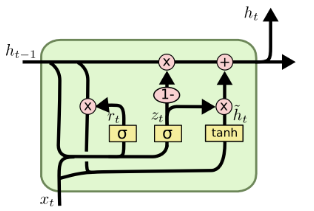
\includegraphics[width=6.0in]{../images/GRU}}
\centerline{{\huge [Christopher Olah]}}

\slide{Long Short Term Memory (LSTM)}
\centerline{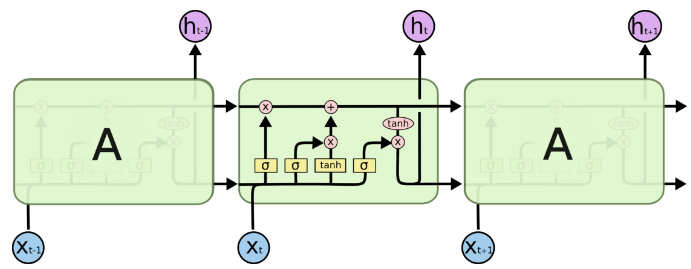
\includegraphics[width=3.5in]{../images/LSTM}}
\centerline{{\large [figure: Christopher Olah]}}

\centerline{\Large [LSTM: Hochreiter\&Shmidhuber, 1997]}

\slide{UGRNN vs. GRUs vs. LSTMs}

\vfill
In class projects from previous years, GRUs consistently outperformed LSTMs.

\vfill
A systematic study [Collins, Dickstein and Sussulo 2016] states:

\begin{quotation}
  Our results point to the GRU as being the most learnable of gated RNNs for shallow architectures, followed by the UGRNN.
\end{quotation}

\slideplain{END}

}
\end{document}
